\section{Principe}
The principle of the optical design to be realized is schematized on the figure \ref{fig:OpticalPrincipe}.\bigbreak
The output beam of the telescope must be made parallel before the system can be installed. Once the beam is parallel,
a mask composed of 2 equal openings will limit it. This mask correspond to the entry of the system.\newline
The beam will enter to a prism which will deflect the beams to a lens.
The lens will intersept the 2 beams and allow to focus them on a sensor (BW camera).
\begin{figure}[H]
    \centering
    \includegraphics[scale=0.7]{assets/figures/Optical Design/Schéma optique.png}
    \caption{Optical schematic principe}
    \label{fig:OpticalPrincipe}
\end{figure}
\newpage
%====================================================================================================
%====================================================================================================
% Drawing rays with matlab
%====================================================================================================
%====================================================================================================
\section{Drawing rays with matlab}
This part will correspond to the mathematical research to draw the rays on a matlab program. To simplify the program,
the chosen method is to draw lines through 2 points. The calculated points are the following:
\begin{enumerate}
    \item Prism entry = ($X_{PE1,2,3,4},Y_{PE1,2,3,4}$)
    \item Prism exit = ($X_{PO1,2,3,4},Y_{PO1,2,3,4}$)
    \item Lens entry/exit = ($X_{L1,2,3,4},Y_{L1,2,3,4}$)
    \item Screen entry = ($X_{S12,34},Y_{S12,34}$)
\end{enumerate}
Known data :
\begin{itemize}
    \item Prism angle = $\alpha$ [$\deg$] (converted into radian for the equations)
    \item Deflection of the incident beam = $i$ [" arc] (converted into radian for the equations)
    \item focal lens = $F$ [mm]
    \item Hole diameter = $d$ [mm]
    \item Distance betweeen two holes = $e$ [mm]
    \item Distance between the prism and the lens = $E$ [mm]
    \item Refractive index of the prism = $n_p$ [-]
    \item Prism width = $t_c$ [mm]
    \item Prism height = $h$ [mm]
\end{itemize}
Needed data :
\begin{itemize}
    \item Screen height = $H$ [mm]
    \item System length = $L$ [mm]
\end{itemize}
\newpage
%====================================================================================================
% Prism
%====================================================================================================
\subsection{Prsim}
\begin{figure}[H]
    \centering
    \includegraphics[scale=0.8]{assets/figures/Optical Design/Schéma prisme.png}
    \caption{Schematic of drawing rays at the input of the prism}
    \label{fig:Prism_Schematic}
\end{figure}
First, set the X and Y input coordinates.
\begin{equation}
    X_{PE1} = X_{PE2} = X_{PE3} = X_{PE4}
\end{equation}
\begin{equation}
    Y_{PE1} = \frac{e + d}{2} \newline
    Y_{PE2} = \frac{e - d}{2} \newline
    Y_{PE3} = \frac{-e - d}{2} \newline
    Y_{PE4} = \frac{-e + d}{2}
\end{equation}
Using Snell's law and the relationships between the angles, the exit angle can be determined.
\begin{equation}
    r = \arcsin(\frac{\sin(i)}{n_p})
\end{equation}

\begin{equation}
    \beta = \arcsin(n_p*\sin(\alpha-\arcsin(\frac{\sin(i)}{n_p})))-\alpha
\end{equation}
To find the output values, the affine line function (\ref{eq:DoiteAffine}) is used.
This requires knowledge of the slopes and offsets of the straight lines (beam + prism output face).
\begin{equation}
    m_1 = \frac{-1}{\tan(\frac{\pi}{2}-r)}\newline
    m_2 = \frac{-1}{\tan(\alpha)}
\end{equation}
\begin{equation}
    m_3 = \frac{-1}{\tan(\frac{\pi}{2}-r)}\newline
    m_4 = \frac{1}{\tan(\alpha)}
\end{equation}
\begin{equation}
    b_1 = Y_{PE1}-X_{PE1}*m_1\newline
    b_2 = Y_{PE2}-X_{PE2}*m_2\newline
    b_{1s} = \frac{h}{2}-t_e*m_2
\end{equation}
\begin{equation}
    b_3 = Y_{PE3}-X_{PE3}*m_3\newline
    b_4 = Y_{PE4}-X_{PE4}*m_4\newline
    b_{2s} = \frac{-h}{2}-t_e*m_4
\end{equation}
Now that the line parameters are known, the X and Y output points of each beam can be calculated.
\begin{equation}
    X_{PO1} = \frac{b_{1s}-b_1}{m_1-m_2}\newline
    Y_{PO1} = X_{PE1}*m_1+b_{1s}
\end{equation}
\begin{equation}
    X_{PO2} = \frac{b_{1s}-b_2}{m_1-m_2}\newline
    Y_{PO2} = X_{PE2}*m_2+b_{1s}
\end{equation}
\begin{equation}
    X_{PO3} = \frac{b_{2s}-b_1}{m_1-m_2}\newline
    Y_{PO3} = X_{PE1}*m_1+b_{1s}
\end{equation}
\begin{equation}
    X_{PO2} = \frac{b_{1s}-b_2}{m_1-m_2}\newline
    Y_{PO2} = X_{PE2}*m_2+b_{1s}
\end{equation}
Once the X,Y coordinates of the prism's inputs and outputs are known, it's easy to plot them in matlab (Appendix \ref{App:Matlab}).
%====================================================================================================
% Lens
%====================================================================================================
\subsection{Lens}
\begin{figure}[H]
    \centering
    \includegraphics{assets/figures/Optical Design/Schéma sortie prisme.png}
    \caption{Schematic of drawing rays at the output of the prism}
    \label{fig:PrismLens_Schematic}
\end{figure}
First, let's say :
\begin{equation}
    X_L = E
\end{equation}
With the equation of the affine line (\ref{eq:DoiteAffine}),
where "a" can be determined using trigonometry (\ref{eq:Trigo_tan}),
The offset can be determined using the points previously obtained.
\begin{equation}
    a = \frac{-1}{tan(90-\beta)}
\end{equation}
\begin{equation}
    Y_{out} = a*X_{out} + b ==> b = Y_{out} - a*X_{out}
\end{equation}
We can now pose the equation that determines the $Y_L$ coordinate
\begin{equation}
    Y_{L} = a*X_{L} + b
\end{equation}
Once the X,Y coordinates of the lens's inputs are known, and with the prism's output coordinates, it's easy to plot them in matlab (Appendix \ref{App:Matlab}).
\subsection{Screen}
\begin{figure}[H]
    \centering
    \includegraphics{assets/figures/Optical Design/Schéma Lentille.png}
    \caption{Schematic of drawing rays at the output of the lens}
    \label{fig:Lens_Schematic}
\end{figure}
To begin with, the X coordinate can be set as it corresponds to the focal
point of the lens. Note that this equation is only valid if the lens is approximated to a thin lens.
\begin{equation}
    X = E+F
\end{equation}
Then, thanks to trigonometry (\ref{eq:Trigo_tan}), it is easy to find the coordinates Y
\begin{equation}
    Y = \pm F*tan(\beta)
\end{equation}
Once the X,Y coordinates of the screen's inputs are known, and with the lens's output coordinates, it's easy to plot them in matlab (Appendix \ref{App:Matlab}).
%====================================================================================================
%====================================================================================================
% Limitations
%====================================================================================================
%====================================================================================================
\newpage
\section{Limitations of the system}\label{sec:Opti_Limit}
\subsection{Theoretical ratio for mask}
As stated in the ESO article on DIMM \cite{DIMM_ESO}, the ratio between the diameter of the holes and their spacing must be 5 :
\begin{equation}\label{eq:Opti_Ratio}
    S = D/d = 5
\end{equation}
The mask is dimensioned in section \ref{sec:Opti_Couille} and this ratio has been used in equation \ref{eq:Opti_ratio}.
\subsection{Solar filter}
If sunspot measurements are to be carried out, the telescope will need to be fitted with a sun filter. This filter will
absorb and reflect UV radiation from the source. Using a filter will prevent damage to the telescope and the DIMM attached to it.
The filter used (figure \ref{fig:Opti_Filter}) will be of the same brand as the telescope (MAEDE). It has been specially made for this one.
\begin{figure}[H]
    \centering
    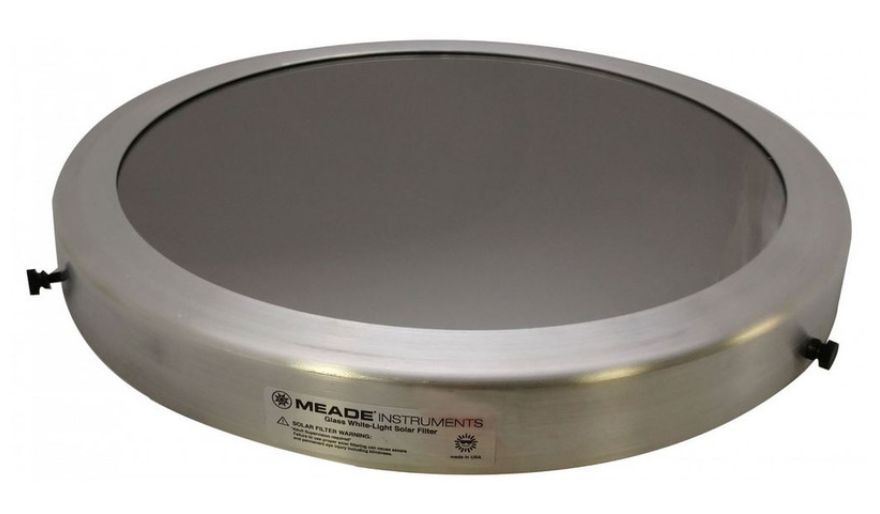
\includegraphics[scale=0.6]{assets/figures/Optical Design/Solar_filter.png}
    \caption{Solar filter}
    \label{fig:Opti_Filter}
\end{figure}
\subsection{Fried parameter}
In order to simplify subsequent calculations, there is a parameter that is constant and varies only with the wavelength that qualifies the turbulence.
This parameter is called the Fried parameter ($r_0$).
This parameter represents a scale of disturbance quality and is expressed in metres :
\begin{itemize}
    \item $r_0$ = 0.02 : \textbf{\textcolor{red}{Ajouter ici}}
    \item $r_0$ = 0.05 : \textbf{\textcolor{red}{Ajouter ici}}
    \item $r_0$ = 0.1 : \textbf{\textcolor{red}{Ajouter ici}}
    \item $r_0$ = 0.2 : \textbf{\textcolor{red}{Ajouter ici}}
\end{itemize}
As the chosen working wavelength is 600nm, the Fried parameter must be adjusted to it as follows:
\begin{equation}
    r_{0-600nm} = r_0*\left(\frac{\lambda_{600}}{500*10^{-9}}\right)^{\frac{6}{5}}
\end{equation}
%====================================================================================================
%====================================================================================================
% Mask sizing
%====================================================================================================
%====================================================================================================
\newpage
\section{Mask sizing}\label{sec:Opti_Couille}
In order to know the mask size required to sample the image, we first need to know the size of the telescope's exit pupil.
\subsection{Sizing of exit pupil}
\begin{figure}[H]
    \centering
    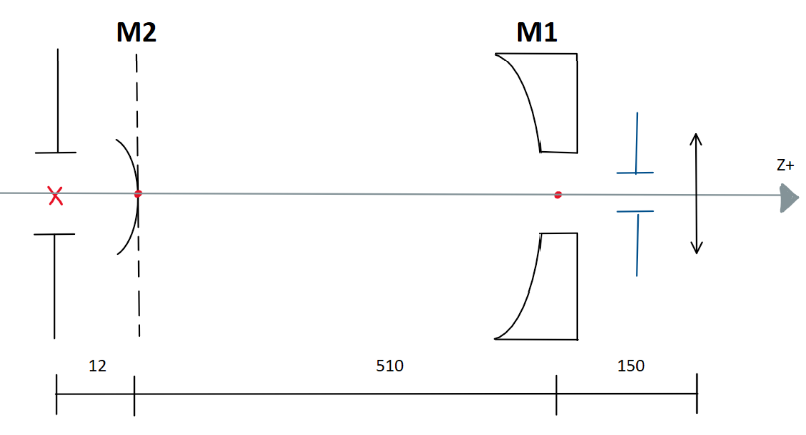
\includegraphics[scale=0.9]{assets/figures/Optical Design/Design_Mask.png}
    \caption{Selected camera}
    \label{fig:Opti_Mask_Diagram}
\end{figure}
Figure \ref{fig:Opti_Mask_Diagram} shows a diagram of the laboratory telescope with its occular.
To determine the position and size of the exit pupil, the following parameters are required:
\begin{itemize}
    \item Aperture diameter (D) : 305mm
    \item Focal length (M1) : -645.2mm
    \item Focal lenght (M2) : 170mm
    \item Focal lenght (Occular) : 26mm
\end{itemize}
The calculation is divided into 3 parts (Object to M1, M1 to M2 and M2 to occular).
To begin with, you need to place the $p_o$ point on the telescope's entrance pupil (Schmidt's Blade) :
\begin{equation}
    p_o^{M1} = -(12+510) = -522mm
\end{equation}
The image plane $p_i$ can then be easily calculated using the law of conjugate foci (\ref{eq:Conjugate}) :
\begin{equation}
    p_i^{M1} = \left(\frac{1}{f^{M1}}-\frac{1}{p_o^{M1}}\right)^{-1} = 2734 mm
\end{equation}
Using $p_o$ and $p_i$, the transverse magnification of the first phase can now be determined :
\begin{equation}
    G_t^{M1} = -\frac{p_i^{M1}}{p_o^{M1}} = 5.24
\end{equation}
For the second phase, you have to start from M1 and go on to M2. To do this, the same calculations have been performed, but this time with :
\begin{equation}
    p_o^{M2} = -(510 + p_i^{M1}) = -3244mm
\end{equation}
With the focal length of M2 and law (\ref{eq:Conjugate}), the second $p_i$ can be found :
\begin{equation}
    p_i^{M2} = \left(\frac{-1}{f^{M2}}-\frac{1}{p_o^{M2}}\right)^{-1} = 162 mm
\end{equation}
Then calculate the magnification of the second phase :
\begin{equation}
    G_t^{M2} = -\frac{p_i^{M2}}{p_o^{M2}} = 0.05
\end{equation}
For the last phase, using the same calculations and posing :
\begin{equation}
    p_o^{OC} = -(510 + p_i^{M2} + 150 + f^{OC}) = -848mm
\end{equation}
The following results for $p_i$ and $G_t$ are :
\begin{equation}
    p_i^{OC} = \left(\frac{-1}{f^{OC}}+\frac{1}{p_o^{OC}}\right)^{-1} = 26.82 mm
\end{equation}
\begin{equation}
    G_t^{OC} = -\frac{p_i^{OC}}{p_o^{OC}} = 0.03
\end{equation}
Now that all the magnifications are known, the total magnification of the telescope and its occular can be calculated :
\begin{equation}
    G_t^{Tot} = G_t^{M1}*G_t^{M2}*G_t^{OC} = \underline{0.008}
\end{equation}
Finally, thanks to the Schmidt blade, which acts as the system's entrance pupil, and the total magnification,
the diameter of the exit pupil can be calculated:
\begin{equation}
    D_p = G_t^{Tot} * D = \underline{2.51mm}
\end{equation}
\subsection{Practical validation}
A practical validation has been carried out. However, the object could not be infinite, as the tests were carried out in the school.
To determine the diameter of the exit pupil, we had to :
\begin{enumerate}
    \item Set up an "artificial" star as far away from the telescope as possible.
    \item Point the telescope at the star and install the occular.
    \item Position your eye on the occular and adjust the telescope's focal length.
    \item Place a grid on the back of the telescope and position it so that the image is sharp (pupil position).
    \item Measure pupil diameter.
\end{enumerate}
These tests gave a pupil diameter of $3 \pm 1$mm. The result is close to what was expected and, taking into account
the uncertainty of the measurement, appears to be fair.
\newline
\textbf{\textcolor{red}{Ajouter image}}
\subsection{Mask sizing}
If the ratio between the diameter of the holes and the distance between them is respected (\ref{eq:Opti_Ratio}), each hole should have a diameter of :
\begin{equation}\label{eq:Opti_ratio}
    D_{Holes} = \frac{D_p}{6} = \underline{0.42mm}
\end{equation}
To ensure that the holes are not on the edge of the pupil, their diameter is set at 0.35mm. With a 0.35mm hole, the distance
between the centers of these 2 holes will be :
\begin{equation}
    d = 5*D_{Holes} = \underline{1.75mm}
\end{equation}
%====================================================================================================
%====================================================================================================
% Camera specifications
%====================================================================================================
%====================================================================================================
\section{Camera specifications}\label{sec:Opti_Cam}
\subsection{Limitations}
In order to determine which sensor will have the right specifications for this application,
several elements will need to be calculated :
\begin{itemize}
    \item Pixel size to ensure an image with sufficient information
    \item Screen size
    \item The size the image will occupy on the sensor
\end{itemize}
\bigbreak
To determine the size of the screen and the pixels required for the image, the previously
calculated magnification and hole size should be used.
The aim is to transfer the mask to the front of the telescope, so as to know the "virtual" size of the mask as
seen through the telescope.
\begin{equation}\label{eq:DMT}
    D_{MT} = \frac{D_{holes}}{G_t} = \frac{0.35}{0.0082} = 42.7mm
\end{equation}
\textbf{\textcolor{red}{Truc du sigma}}
\begin{equation}
    \sigma_T = \sqrt{0.1698*\left(\frac{\lambda}{D_{MT}}\right)^2*\left(\frac{D_{MT}}{r_{0-600nm}}\right)^{\frac{5}{3}}}
\end{equation}
Then simply transform the $\sigma_t$ into arc seconds for the rest of the calculations.
\newline
Once the $\sigma_T$ is known, the fov as seen through the telescope can be determined. In equation \ref{eq:FOV_T}, $D_S$ is the diameter
of the sunspots to be measured (20").
\begin{equation}\label{eq:FOV_T}
    FOV_T = 6 * \sigma_T + D_S
\end{equation}
Once the FOV seen by the telescope is known, this parameter must be transferred to the mask.
\begin{equation}
    FOV_M = FOV_T * G_t^{-1}
\end{equation}
This FOV will be converted into a radiant and can then be transferred to the CMOS sensor
using the lens focal length ($F$) determined in section \ref{sec:Opti_Lens}.
\begin{equation}
    FOV_S = FOV_M * F
\end{equation}
Finally, the three elements listed at the beginning of this section can be calculated.
\begin{itemize}
    \item The maximum pixel size of the CMOS sensor must respect Niquist's theorem.
          \begin{equation}
              pixel_{max} = \frac{\lambda*F}{2*D_{holes}}
          \end{equation}
    \item The number of pixels in an image will be :
          \begin{equation}
              N_{p} = \frac{FOV_S}{pixel_{max}}
          \end{equation}
    \item The minimum screen size required to view the 2 images (assuming they are centered) is :
          \begin{equation}
              Screen_{Size} = (\frac{H}{pixel_{max}}+ N_{p}*2);
          \end{equation}
\end{itemize}
For the 3 points above, calculations were performed using matlab (Appendix \ref{App:Matlab}) and worst-case scenarios
were considered. Calculations were made for a value of $r_0$ ranging from 0.02m to 0.2m.
Based on these calculations, the following results were obtained:
\begin{itemize}
    \item Maximum pixel size : 15 [$\mu$m]
    \item Minimum screen size : 164 [pixel]
    \item Size of one image : 17 [pixel]
\end{itemize}
\subsection{Choice}
With the specifications calculated above and after some research, the camera shown in figure 2 was chosen.
\begin{figure}[H]
    \centering
    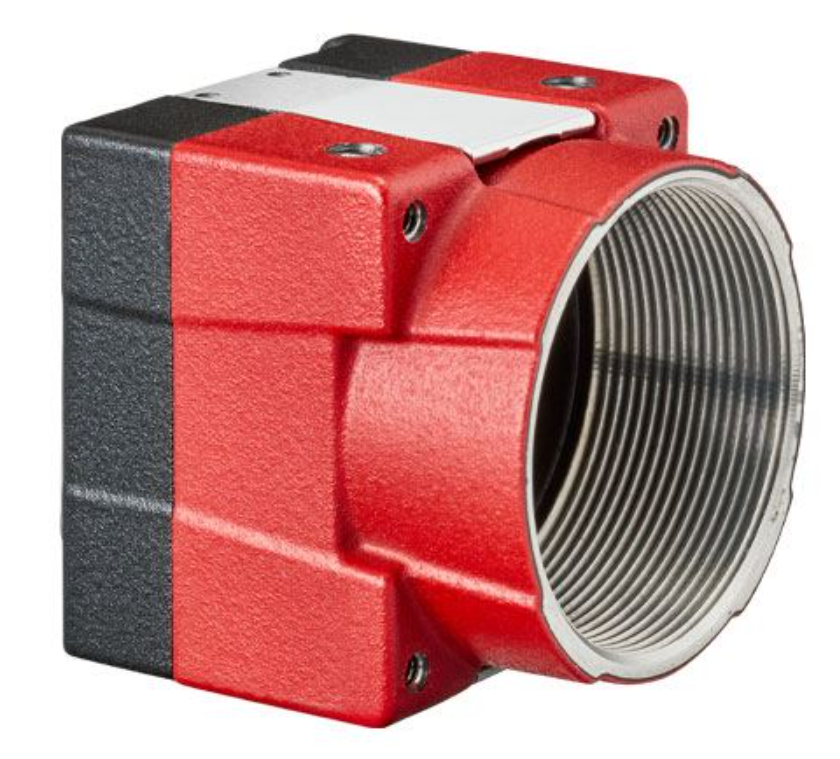
\includegraphics[scale=0.35]{assets/figures/Mechanical Design/Camera.png}
    \caption{Selected camera}
    \label{fig:Camera2}
\end{figure}
The camera in figure \ref{fig:Camera2} is an Allied vision camera (Alvium 1800 U-052m). This camera is
equipped with a monochromatic CMOS sensor (Sony IMX426). Its pixels are 9x9 [$mu$m], its size is 816x624 [pixel]
and this camera is capable of exposure times from 21 $mu$s to 10s.
\bigbreak
With this camera, an image will take up around 28 pixels and the total image will be 250 pixels long.
If the total image is centered on the sensor, camera orientation will have no effect on the measurement.
The image should always be on the sensor.
%====================================================================================================
%====================================================================================================
% Lens selection
%====================================================================================================
%====================================================================================================
\newpage
\section{Lens selection}\label{sec:Opti_Lens}
The choice of lens is one of the critical elements of this project. Several parameters need to be taken
into account, such as \gls{PSF} on the focal plane, Zernike polynomials and the correct Strehl ratio.
The validation method for the use of a certain lens was a simulation on Zemax.
In order to best reproduce the system, an angle on the incident beam had to be added.
This angle corresponds to the beam deflection produced by the prism. The wavelength will also have to be modified to work at 600nm.
\begin{figure}[H]
    \centering
    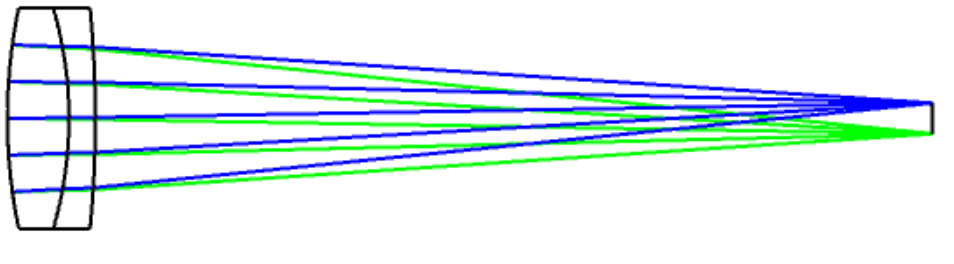
\includegraphics[scale=0.8]{assets/figures/Optical Design/Zemax_RayTrace.png}
    \caption{Drawing of lens rays on Zemax}
    \label{fig:Opti_LensRayTrace}
\end{figure}
In order to maximize the system's critical parameters, it is essential to optimize the system when
the fields have not yet been introduced.
Once the system has been optimized, the beam angle can be entered in the "Data field editor".
\begin{figure}[H]
    \centering
    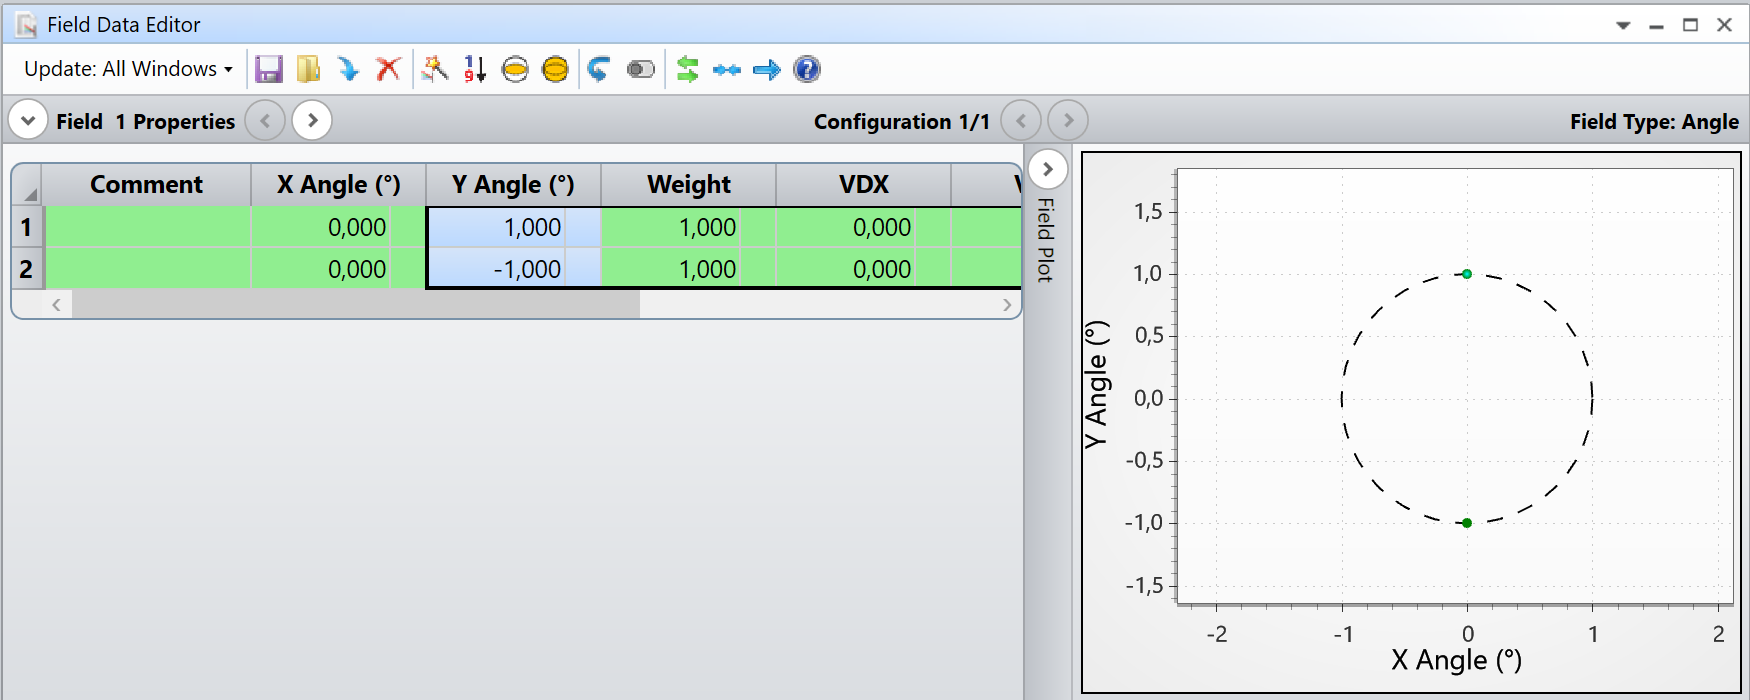
\includegraphics[scale=0.5]{assets/figures/Optical Design/Zemax_FieldEditor.png}
    \caption{zemax parameter window : "Field data Editor"}
    \label{fig:Opti_FieldZemax}
\end{figure}
Now that the parameters have been entered, all that remains is to analyze the results.
\newpage
\subsection{Point Spread Function}
The \gls{PSF} is the most critical element of optical design. It determines the image quality of the lens.
A good \gls{PSF} is characterized by a large peak centered in position (0,0) and a low spread of the function.
\newline
In Figure \ref{fig:Opti_ZemaxPSF}, the \gls{PSF} has a correct shape and its maximum rises to 0.875. This \gls{PSF} is completely acceptable
for the DIMM lens. It is that of the lens chosen (F=50mm) with a beam incidence angle of 1$^{\circ}$.
\begin{figure}[H]
    \centering
    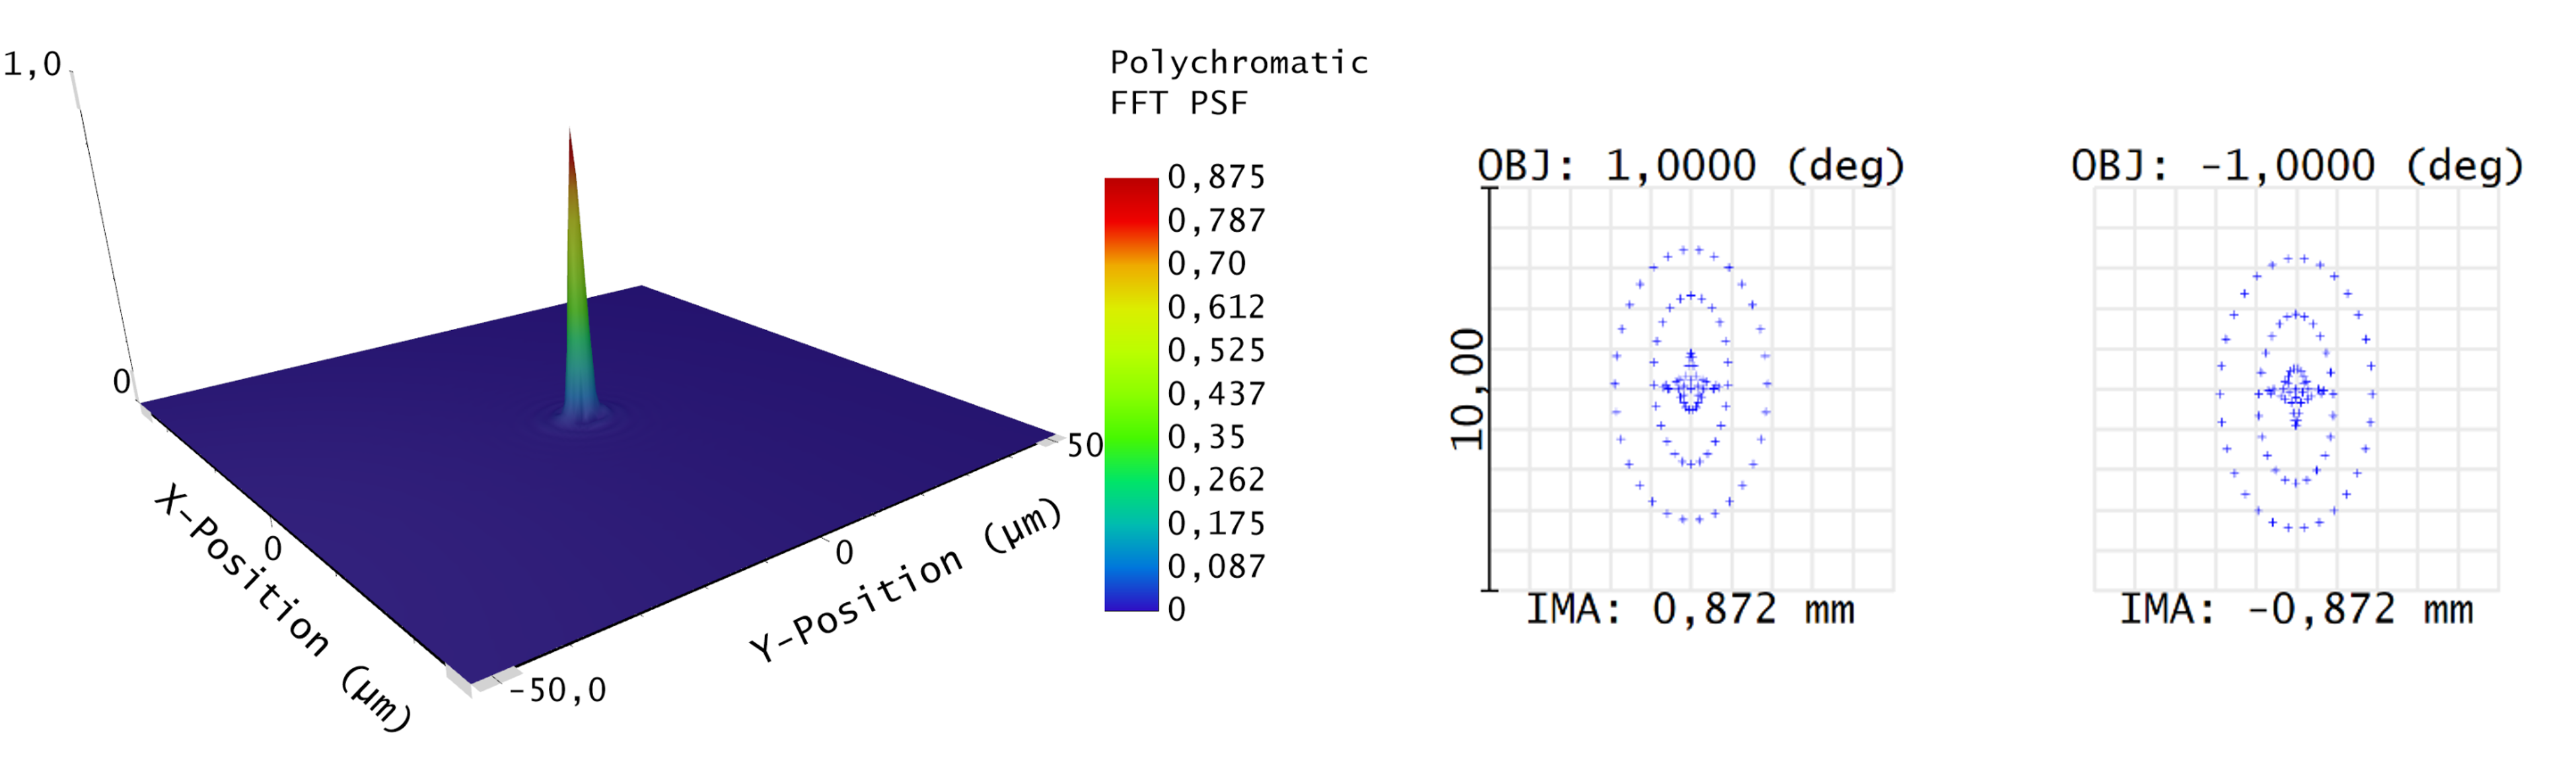
\includegraphics[scale=0.5]{assets/figures/Optical Design/Zemax_PSF.png}
    \caption{PSF and Spot diagram for the chosen lens}
    \label{fig:Opti_ZemaxPSF}
\end{figure}
\subsection{Strehl ratio}
The Strehl ratio compares the peak intensity of the actual focused image to that of an ideal,
diffraction-limited image formed by a perfect optical system. A Strehl ratio of 1 indicates perfect performance,
while lower values indicate the presence of aberrations.
\begin{figure}[H]
    \centering
    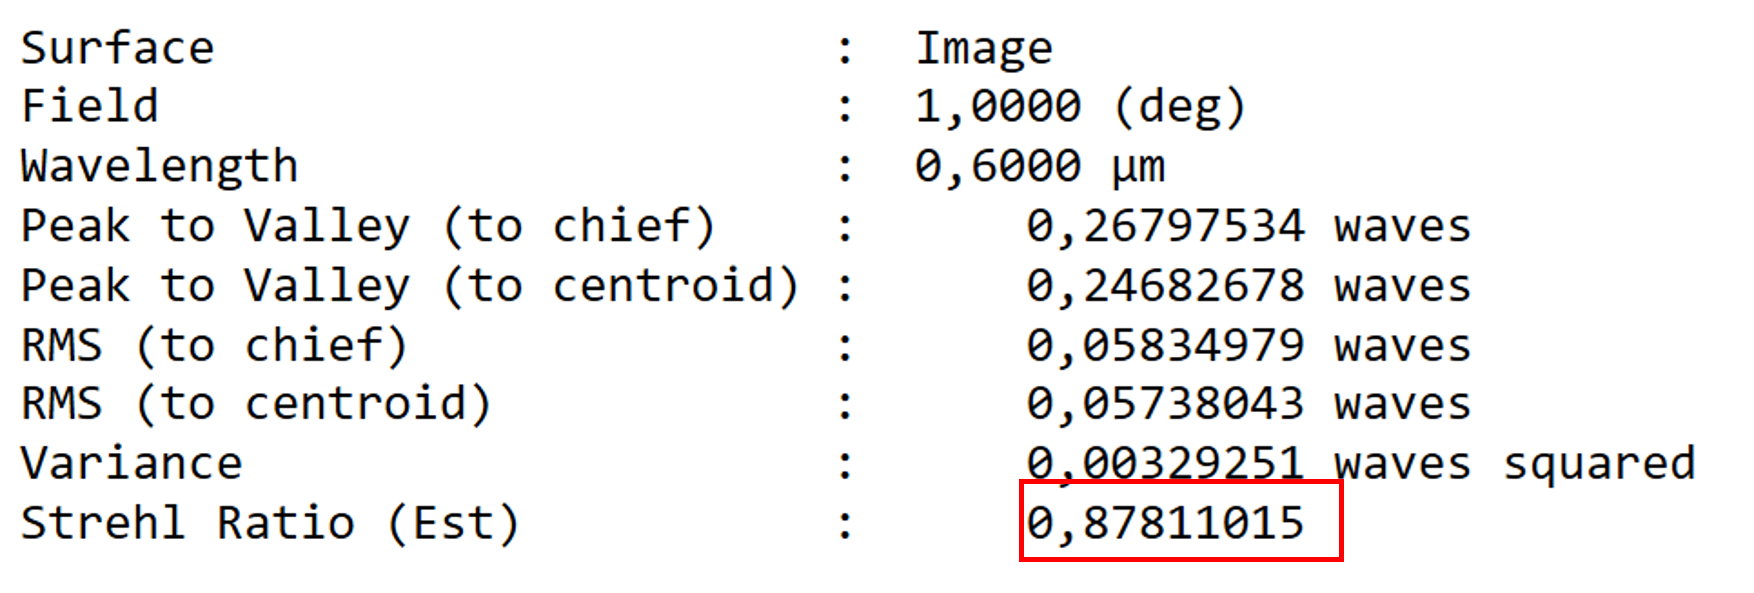
\includegraphics[scale=0.8]{assets/figures/Optical Design/Zemax_Strehl.png}
    \caption{Strehl lens ratio}
    \label{fig:Opti_ZemaxStrehl}
\end{figure}
In this case, the strehl ratio is 0.878. This indicates that the lens, in its configuration,
has the necessary parameters for this application.
\newpage
\subsection{Zernike polynomials}
Zernike polynomials define the output wavefront of a system. Each coefficient of this polynomial refers to an
aberration in the optical system. The aim is to minimize these polynomials to obtain, in the best (theoretical)
case, an image that is completely identical to the object. For this project, the polynomials that must be as small as possible are :
\begin{itemize}
    \item \textbf{2-3} : Tilt : The higher this parameter, the greater the tilt on the X and Y axes. Too high a tilt will distort
          the image and sunspot detection may not work.
    \item \textbf{4}   : Defocus : It happens when an optical system fails to converge light rays onto a single point. The higher the
          defocus setting, the greater the contrast between blur and sharpness.
    \item \textbf{5-6} : Astigmatism : This is the most important parameter in this project. Astigmatism compromises image
          sharpness when the beams are far from the optical axis. The appearance of a blur on the final image could compromise the
          measurement. The image would be averaged, in which case the seeing would not be fixed.
    \item \textbf{7-8} : Sphericity : Spherical aberration is an optical aberration that occurs when a lens or mirror fails to focus all
          incoming light rays to a single point. It causes blurring and loss of sharpness in the resulting image. Once again, if the measurement
          is blurred, this will result in a seeing that has not been fixed and therefore an inaccurate measurement.
\end{itemize}
\begin{figure}[H]
    \centering
    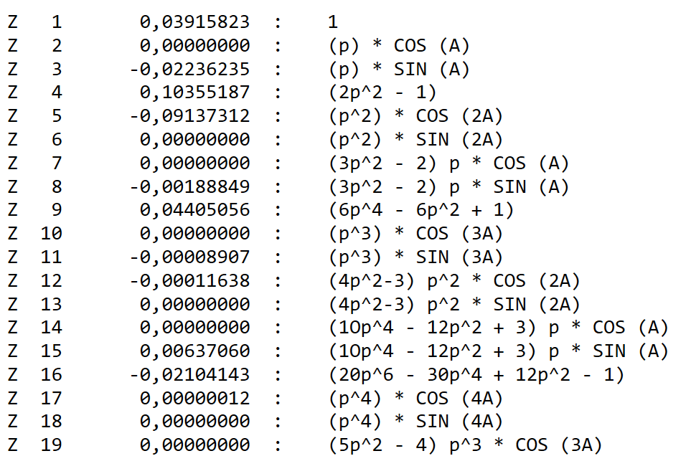
\includegraphics[scale=0.9]{assets/figures/Optical Design/Zemax_Zernik.png}
    \caption{Lens zernike polynomials}
    \label{fig:Opti_ZemaxZernik}
\end{figure}
\textbf{\textcolor{red}{Expliquer pourquoi c'est bien}}
\subsection{Final choice}
\begin{figure}[H]
    \centering
    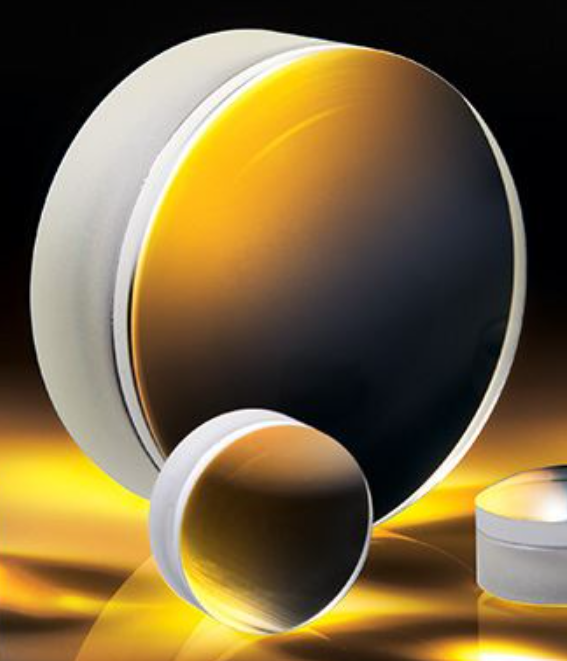
\includegraphics[scale=0.7]{assets/figures/Mechanical Design/Lentille.png}
    \caption{Lens choosed}
    \label{fig:Opti_Lens}
\end{figure}
The lens chosen for the system is the one shown in figure \ref{fig:Opti_Lens}, and was selected in combination with all
the other elements as explained in section \ref{sec:Opti_Limit}. The lens has the following characteristics:
\begin{itemize}
    \item Type: Achromatic Lens
    \item Effective Focal Length EFL (mm): 50.00
    \item Wavelength Range (nm): 425 - 675
    \item Coating Specification: Ravg ≤0.4\% @ 425 - 675nm
\end{itemize}
%====================================================================================================
%====================================================================================================
% Prism selection
%====================================================================================================
%====================================================================================================
\newpage
\section{Prism selection}\label{sec:Opti_Prism}
As far as the prism is concerned, the limiting factor is the beam exit angle. This angle will influence the choice of lens.
\newline
The primary objective was to create a custom-made prism in the shape of a square-based pyramid. This would have made it
possible to produce 4 images and thus refine the measurement. After several requests for bids, it turned out that a custom-made
square-based prism was too expensive ($\approx$ 4000 CHF). After that, it was decided to re-tender with a 2-sided prism, but the price
didn't come down. The final solution was to buy a commercially available prism, produced in large numbers. However, this type of
prism is only available in circular format. We therefore had to find a way of adapting and mounting it (Section \ref{sec:prisms}).
\bigbreak
The search for prisms was therefore carried out on the Edmund optics website.
This supplier offers a wide range of prisms with treatments equivalent to the lens treatment.
Available prisms offer beam exit angles ranging from 0.5$^{\circ}$ to 15$^{\circ}$.
\newline
As stated in section \ref{sec:Opti_Lens}, the prism must produce an angle of 1$^{\circ}$ at its exit to correpsond with the
choice of lens. The prism shown in figure 2 was therefore chosen.
\begin{figure}[H]
    \centering
    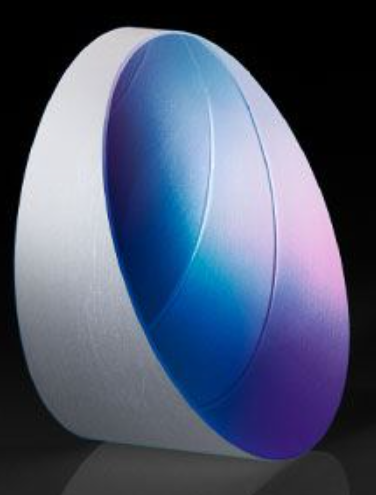
\includegraphics[scale=0.8]{assets/figures/Mechanical Design/Prisme_obtenu.png}
    \caption{Prism choosed}
    \label{fig:Opti_Prism}
\end{figure}
The prism chosen has the following characteristics:
\begin{itemize}
    \item Wavelength Range (nm): 425 - 675
    \item Surface Flatness (P-V): λ/10
    \item Ray Deviation @ 633nm ($^{\circ}$): 1.00
    \item Substrate: N-BK7
    \item Wedge Angle: 1$^{\circ}$ 56'
\end{itemize}
%====================================================================================================
%====================================================================================================
% Limitation
%====================================================================================================
%====================================================================================================
\newpage
\section{Design method}
The overall dimensioning of the optical system can be realized as a kind of loop, where each
parameter is linked to another component of the system. As shown in Figure \ref{fig:Opti_DiagrammChoices} :
\begin{itemize}
    \item The diameter of the holes on the mask and their spacing will have a bearing on the distance available between the prisms.
    \item The angle of incidence of the prisms will have a bearing on the total length of the system, as well as the \Gls{PSF} of the lens.
    \item The focal length of the lens will be related to the overall length of the system, as will the minimum pixel size on the CMOS sensor.
\end{itemize}
Each element will therefore have an influence on a component of the system. The aim is to find the perfect combination of efficiency,
compactness and reliability. If all the components fit together, but it's impossible to find the right pixel size,
you'll have to start all over again.
Numerous tests and simulations were carried out to find the right combination. However, once the right combination has been found,
it is necessary to check that the components are available on the market, to avoid incurring additional costs.
\begin{figure}[H]
    \centering
    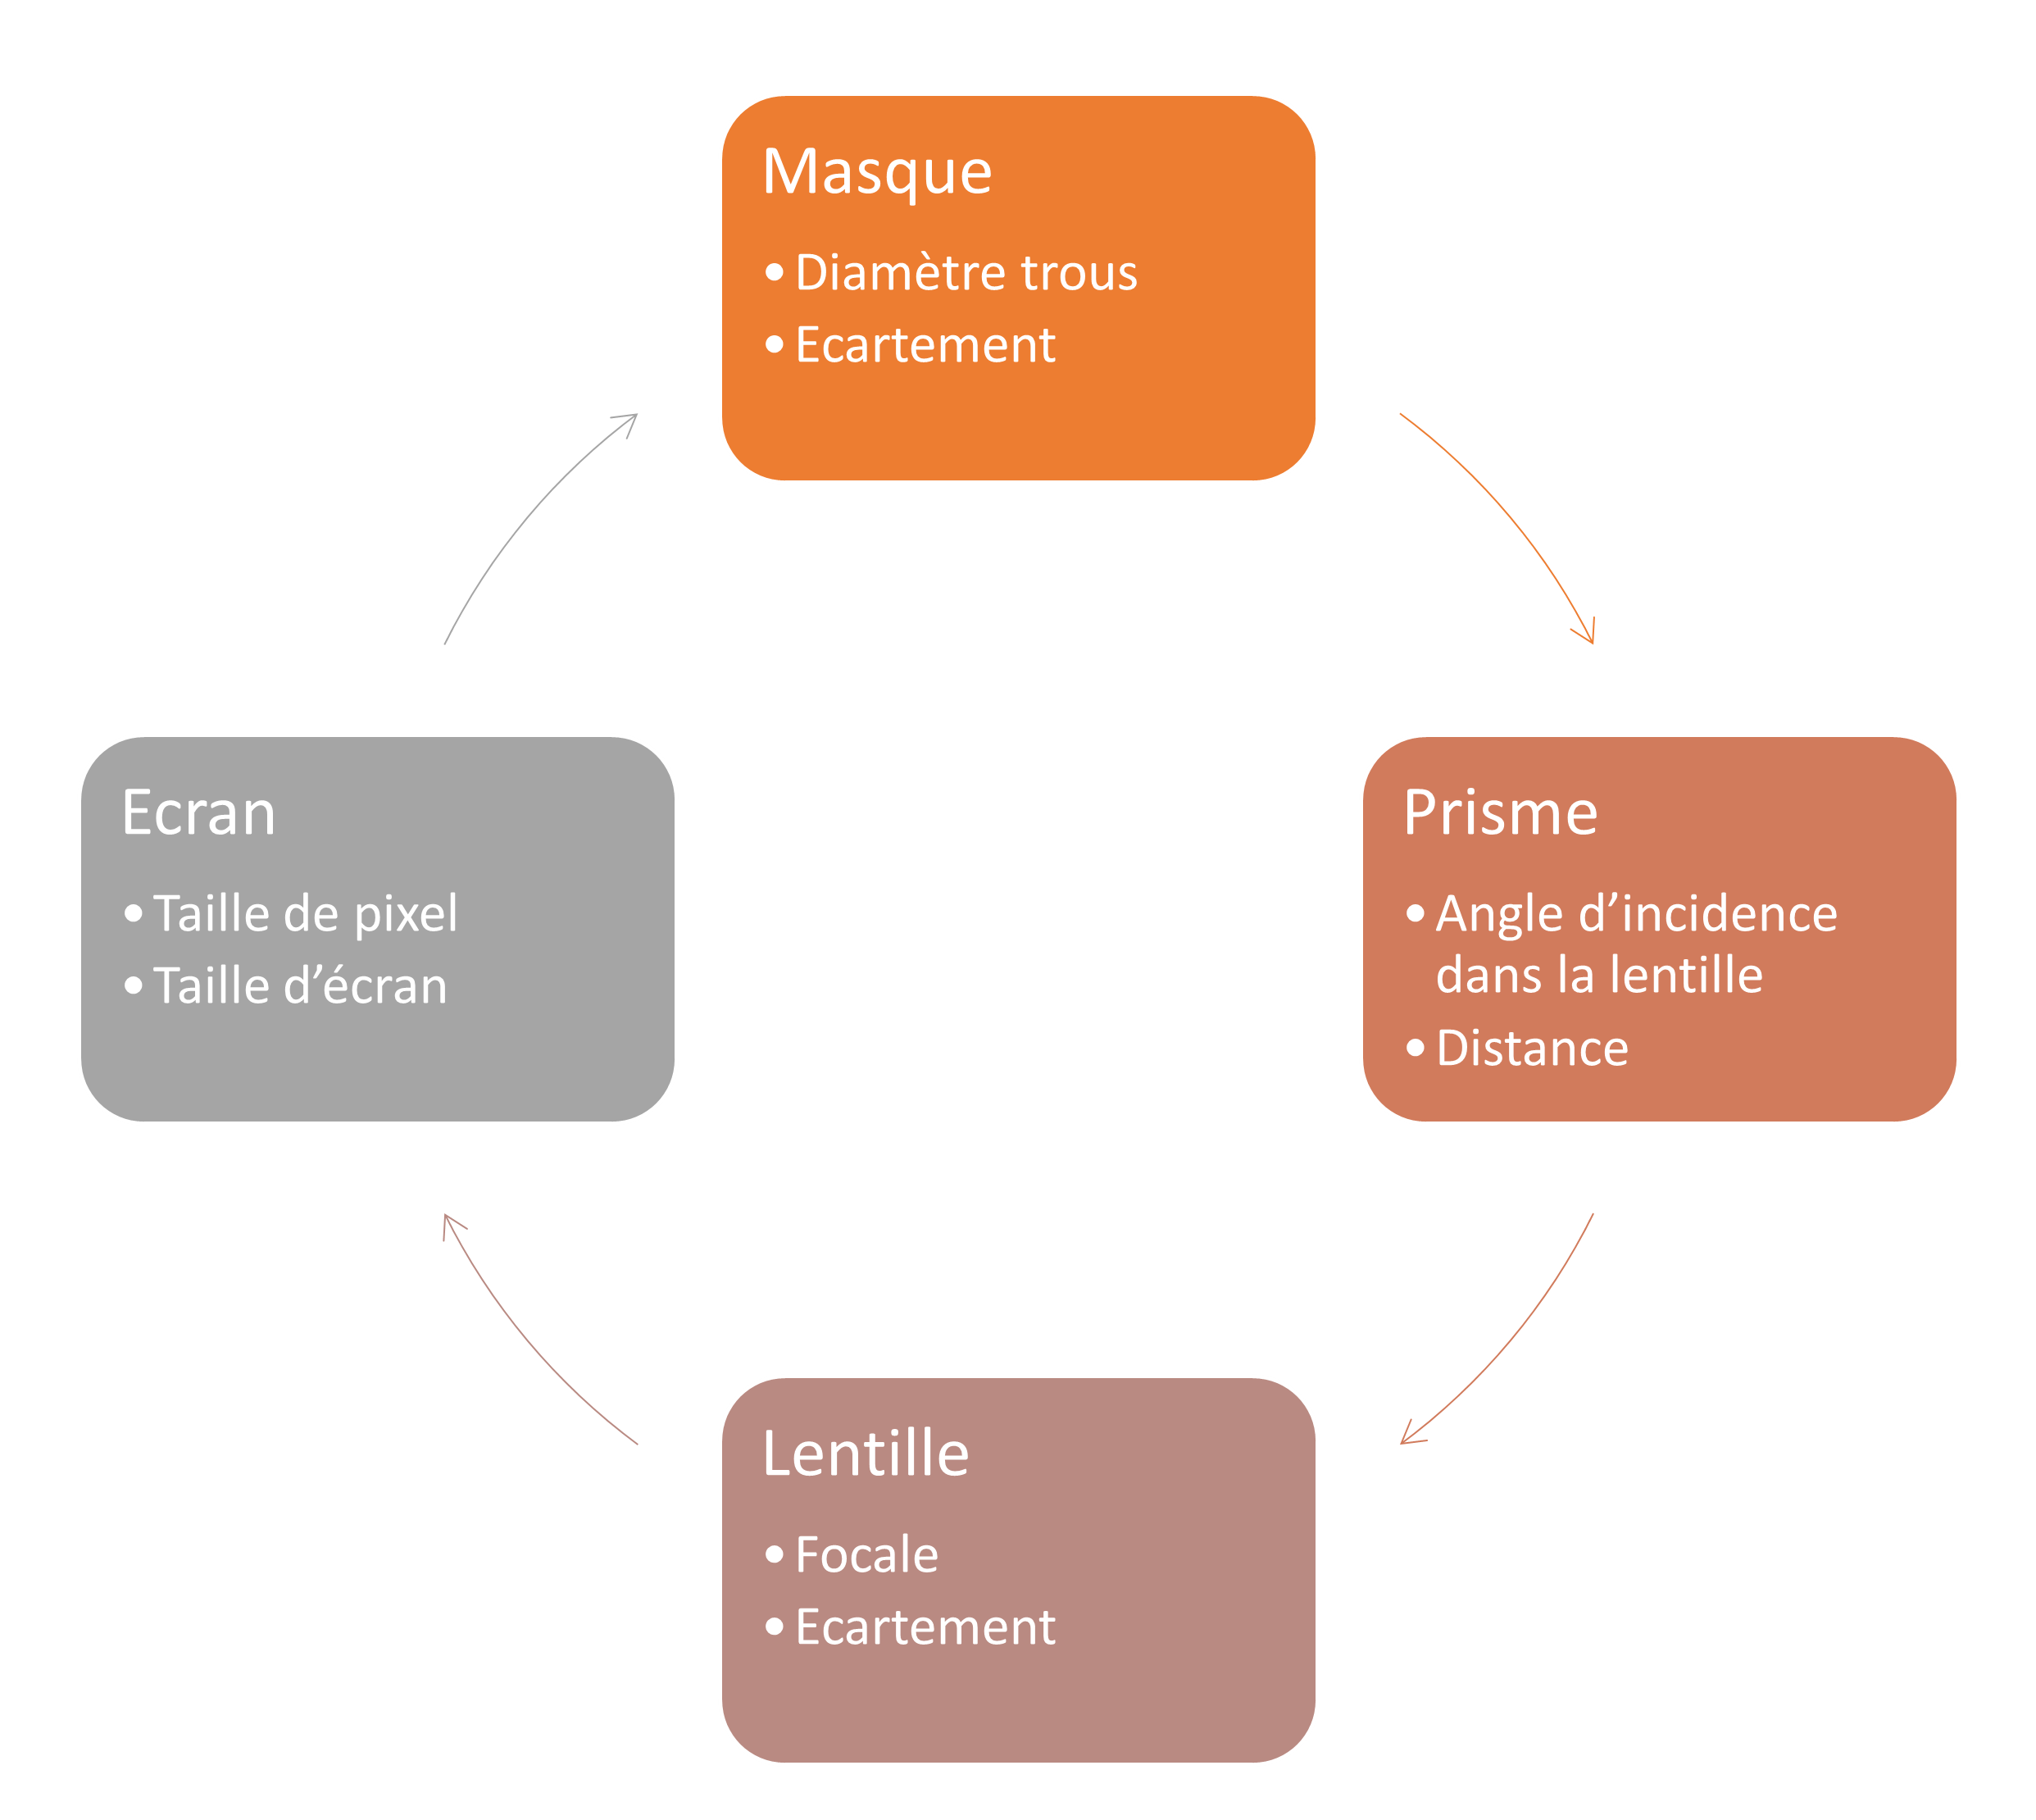
\includegraphics[scale=0.25]{assets/figures/Optical Design/Diagramme_Limitation.png}
    \caption{Component selection diagram}
    \label{fig:Opti_DiagrammChoices}
\end{figure}